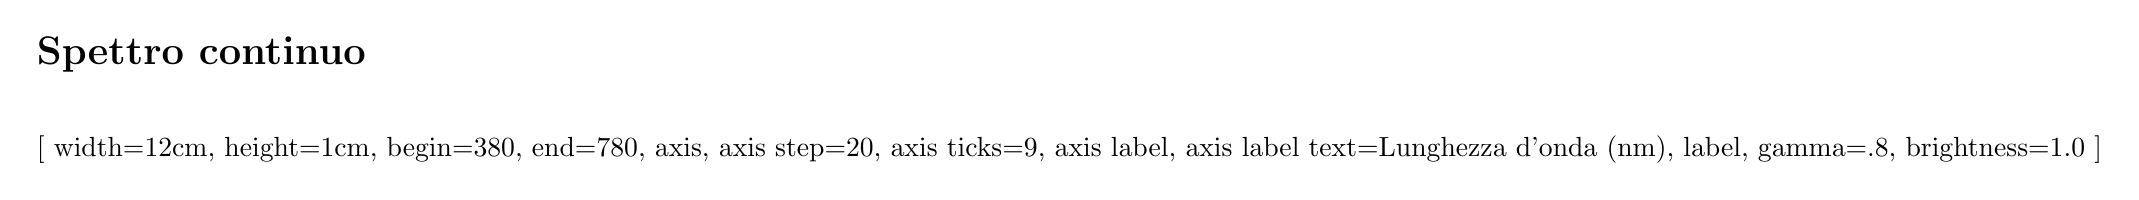
\begin{tikzpicture}[x=1cm,y=1cm]

  % Parametri condivisi
  \def\W{12cm}     % larghezza pannelli
  \def\H{1cm}      % altezza pannelli
  \def\G{0.8cm}    % gap verticale tra i pannelli
  \def\lambdaMin{380}
  \def\lambdaMax{780}

  % Punto di riferimento comune (sinistra dei pannelli)
  \coordinate (left) at (0,0);

  %--------------------------
  % Spettro continuo
  %--------------------------
  \node[anchor=west] at ([yshift=1.2cm]left) {\Large\bfseries Spettro continuo};

  %--------------------------
  % Pannello superiore: spettro continuo
  %--------------------------
  \node[anchor=west] (spec) at (left) {%
    \pgfspectra[
      width=\W,
      height=\H,
      begin=\lambdaMin, end=\lambdaMax,
      axis, axis step=20, axis ticks=9,
      axis label, axis label text={Lunghezza d'onda (nm)},
      label,
      gamma=.8, brightness=1.0
    ]%
  };
\end{tikzpicture}
  %--------------------------
  % Spettro emesso
  %--------------------------
\vfill

\begin{tikzpicture}[x=1cm,y=1cm]
  % Parametri condivisi
  \def\W{12cm}     % larghezza pannelli
  \def\H{1cm}
  \def\G{0.8cm}    % gap verticale tra i pannelli
  \def\lambdaMin{380}
  \def\lambdaMax{780}

\node[anchor=west] at ([yshift=1.2cm]left) {\Large\bfseries Spettro di emissione dell'atomo di idrogeno};

\pgfspectraStyle[
  axis,                 % mostra l'asse delle λ
  begin=\lambdaMin,            % inizio (nm)
  end=\lambdaMax,              % fine (nm) - visibile
  axis step=20,         % passo delle tacche (nm)
  axis ticks=9,         % densità tacche
  axis label,
  axis label text={Lunghezza d'onda (nm)},
  width=\W,     % larghezza della barra
  height=\H,         % altezza della barra
  back=visible20,       % sfondo "arcobaleno" del visibile (30% opacità)
  line width=1pt,       % spessore delle righe di emissione
  gamma=.8              % correzione percettiva del colore (facoltativa)
]

\node[anchor=west] (spec) at ([xshift=0.8cm]left) {\pgfspectra[element=H]};

\end{tikzpicture}

 %--------------------------
  % Spettro uscente
  %--------------------------

\vfill

\begin{tikzpicture}[x=1cm,y=1cm]
  % Parametri condivisi
  \def\W{12cm}     % larghezza pannelli
  \def\H{1cm}
  \def\G{0.8cm}    % gap verticale tra i pannelli
  \def\lambdaMin{380}
  \def\lambdaMax{780}

\node[anchor=west] at ([yshift=1.2cm]left) {\Large\bfseries Linee di assorbimento};

\pgfspectraStyle[
  axis,                 % mostra l'asse delle λ
  begin=\lambdaMin,            % inizio (nm)
  end=\lambdaMax,              % fine (nm) - visibile
  axis step=20,         % passo delle tacche (nm)
  axis ticks=9,         % densità tacche
  axis label,
  axis label text={Lunghezza d'onda (nm)},
  width=\W,     % larghezza della barra
  height=\H,         % altezza della barra
  back=visible20,       % sfondo "arcobaleno" del visibile (30% opacità)
  line width=1pt,       % spessore delle righe di emissione
  gamma=.8,              % correzione percettiva del colore
]

\node[anchor=west] (spec) at ([xshift=0.8cm]left) {\pgfspectra[element=H, absorption]};

\end{tikzpicture}
